\section{Noticia de ``The economics of prison gangs''}
\begin{itemize}
    \item Es atractiva la idea de estar en una pandilla, proveen protección, y otras cosas.
    \item Las pandillas es un resultado de coordinación, las prisiones no cubren la protección del prisionero.
    \item \emph{\textbf{Observación: }La función económica de las pandillas:}
        \begin{enumerate}
            \item Contrabando: Principalmente las drogas \emph{\textbf{Recordar lo siguiente:}26\%  el contrabando es drogas}.
            \item Sistema comunitario: Las pandillas proveen un sistema pseudo-jurídico, se cumplen las cosas que se dicen porque de lo contrario se ejerce coacción. 
            \item Tiempo de calidad: proveen ``amenidades''
            \item Comportamiento: a ellos les genera pérdidas la violencia por ende su sistema jurídico incentiva en contra de la violencia pero indudablemente proveen una institución de coacción.
        \end{enumerate}
    
    \item La economía de las pandilla es similar al trueque.
    \item \emph{\textbf{Observación: }Se tiende a preferir en estados unidos por razas.}
\end{itemize}

%%%%%%%%%%%%%%%%%%%%%%%%%%%%%%%%%%%%%%%%%%%%%%%%%%%%%%%%%%%%%%%%%%%%%%%%%%%%%%%%%%%%%%%%%%%%%%%%
\section{Discusión de clase}
\begin{enumerate}
    \item Continuación de la ley de Gresham, \emph{Citación:``Cuando \textbf{no} hay tipo de cambio fijo se da el caso que la moneda buena expulsa a la mala"}, pasa el caso descrito anteriormente y surge un problema, que se hay dinero con diferente unidad de cuenta.
    \item La autoridad quiere solucionar esto entonces impone un tipo de cambio y lo que ocurre es que hacen circular la moneda mala.
    \item Tiende a ocurrir: la moneda que la ley sobre evalúa se va, \emph{Citación:``Cuando te ponen una opción de pagar menos o más vas a pagar menos, entonces tiende a desaparecer la moneda buena y la mala sube por inflación"}.
    \item \textbf{En términos de dinero el bien malo tiende a circular y la buena se desaparece.}
    \item Uno puede rastrear monedas en Europa tan solo viendo los tipos de cambio en una región.
\end{enumerate}

%%%%%%%%%%%%%%%%%%%%%%%%%%%%%%%%%%%%%%%%%%%%%%%%%%%%%%%%%%%%%%%%%%%%%%%%%%%%%%%%%%%%%%%%%%%%%%%%

\subsection{La ley de Thiers}
\begin{enumerate}
    \item Es el reverso de la ley de Gresham, sostiene lo opuesto de la ley de Gresham.
    \item Dinamicas de hiperinflación, \textbf{Nos preguntamos:} ¿Por qué pasa la hiper invlación?
        \begin{itemize}
            \item \emph{\textbf{Definición de ``hiperinflación":} que el IPC suba más de 50\% mensual}
            \item  Hiperinflación:
                \[
                    \text{Déficit fiscal} \longrightarrow \underbrace{\text{Incremento cantidad dinero}}_{\text{Ver: Causas hiper-inflatorias}} \longrightarrow \underbrace{\text{Hiperinflación}}_{\text{IPC} + 50\%} 
                \]

            
            \item La causa de incremento en la cantidad de dinero es que el gobierno no quiere subir los impuestos pero quiere gastar, $\Rightarrow$ imprime dinero.
            \item \emph{\textbf{Recordar lo siguiente:}Cuando se intentó subir el IVA casi hubo una revolución, entonces hay un incentivo a \textbf{gastar sin ingresar} $\Rightarrow$ déficit público $\Rightarrow$ Los bancos centrales imprimen dinero $\Rightarrow$ inflación.}
            \item Para llegar a una hiperinflación el \emph{Déficit fiscal \& el incremento en la cantidad de dinero} tienen que ser muy grandes.
            \item \emph{\textbf{Recordar lo siguiente:}Cuando aumentó los precios en toda Europa, se encontró una gran cantidad de plata y oro entonces hubo un influjo grandísimo de dinero y hubo una ``revolución de los precios'', llegó a ser 1190\% al año. \emph{\textbf{(Paréntesis ``cálculo de esta hiper inflación'':}$(1 + i)^{n}$\textbf{)}}}.
            \item En GT hay una inflación promedio de 5.5\% y en el momento de la ``revolución europea de precios'' la inflación fue de 5.5\% interesante la re-definición de lo que es una hiperinflación hoy en día. 
            \item \textbf{Nos preguntamos:} ¿Qué ocurre con el dinero en una hiper-inflación? \emph{\textbf{La respuesta a esta pregunta es: } que se devalúa hasta casi cero.}
                \begin{figure}[htbp]
                    \centering
                    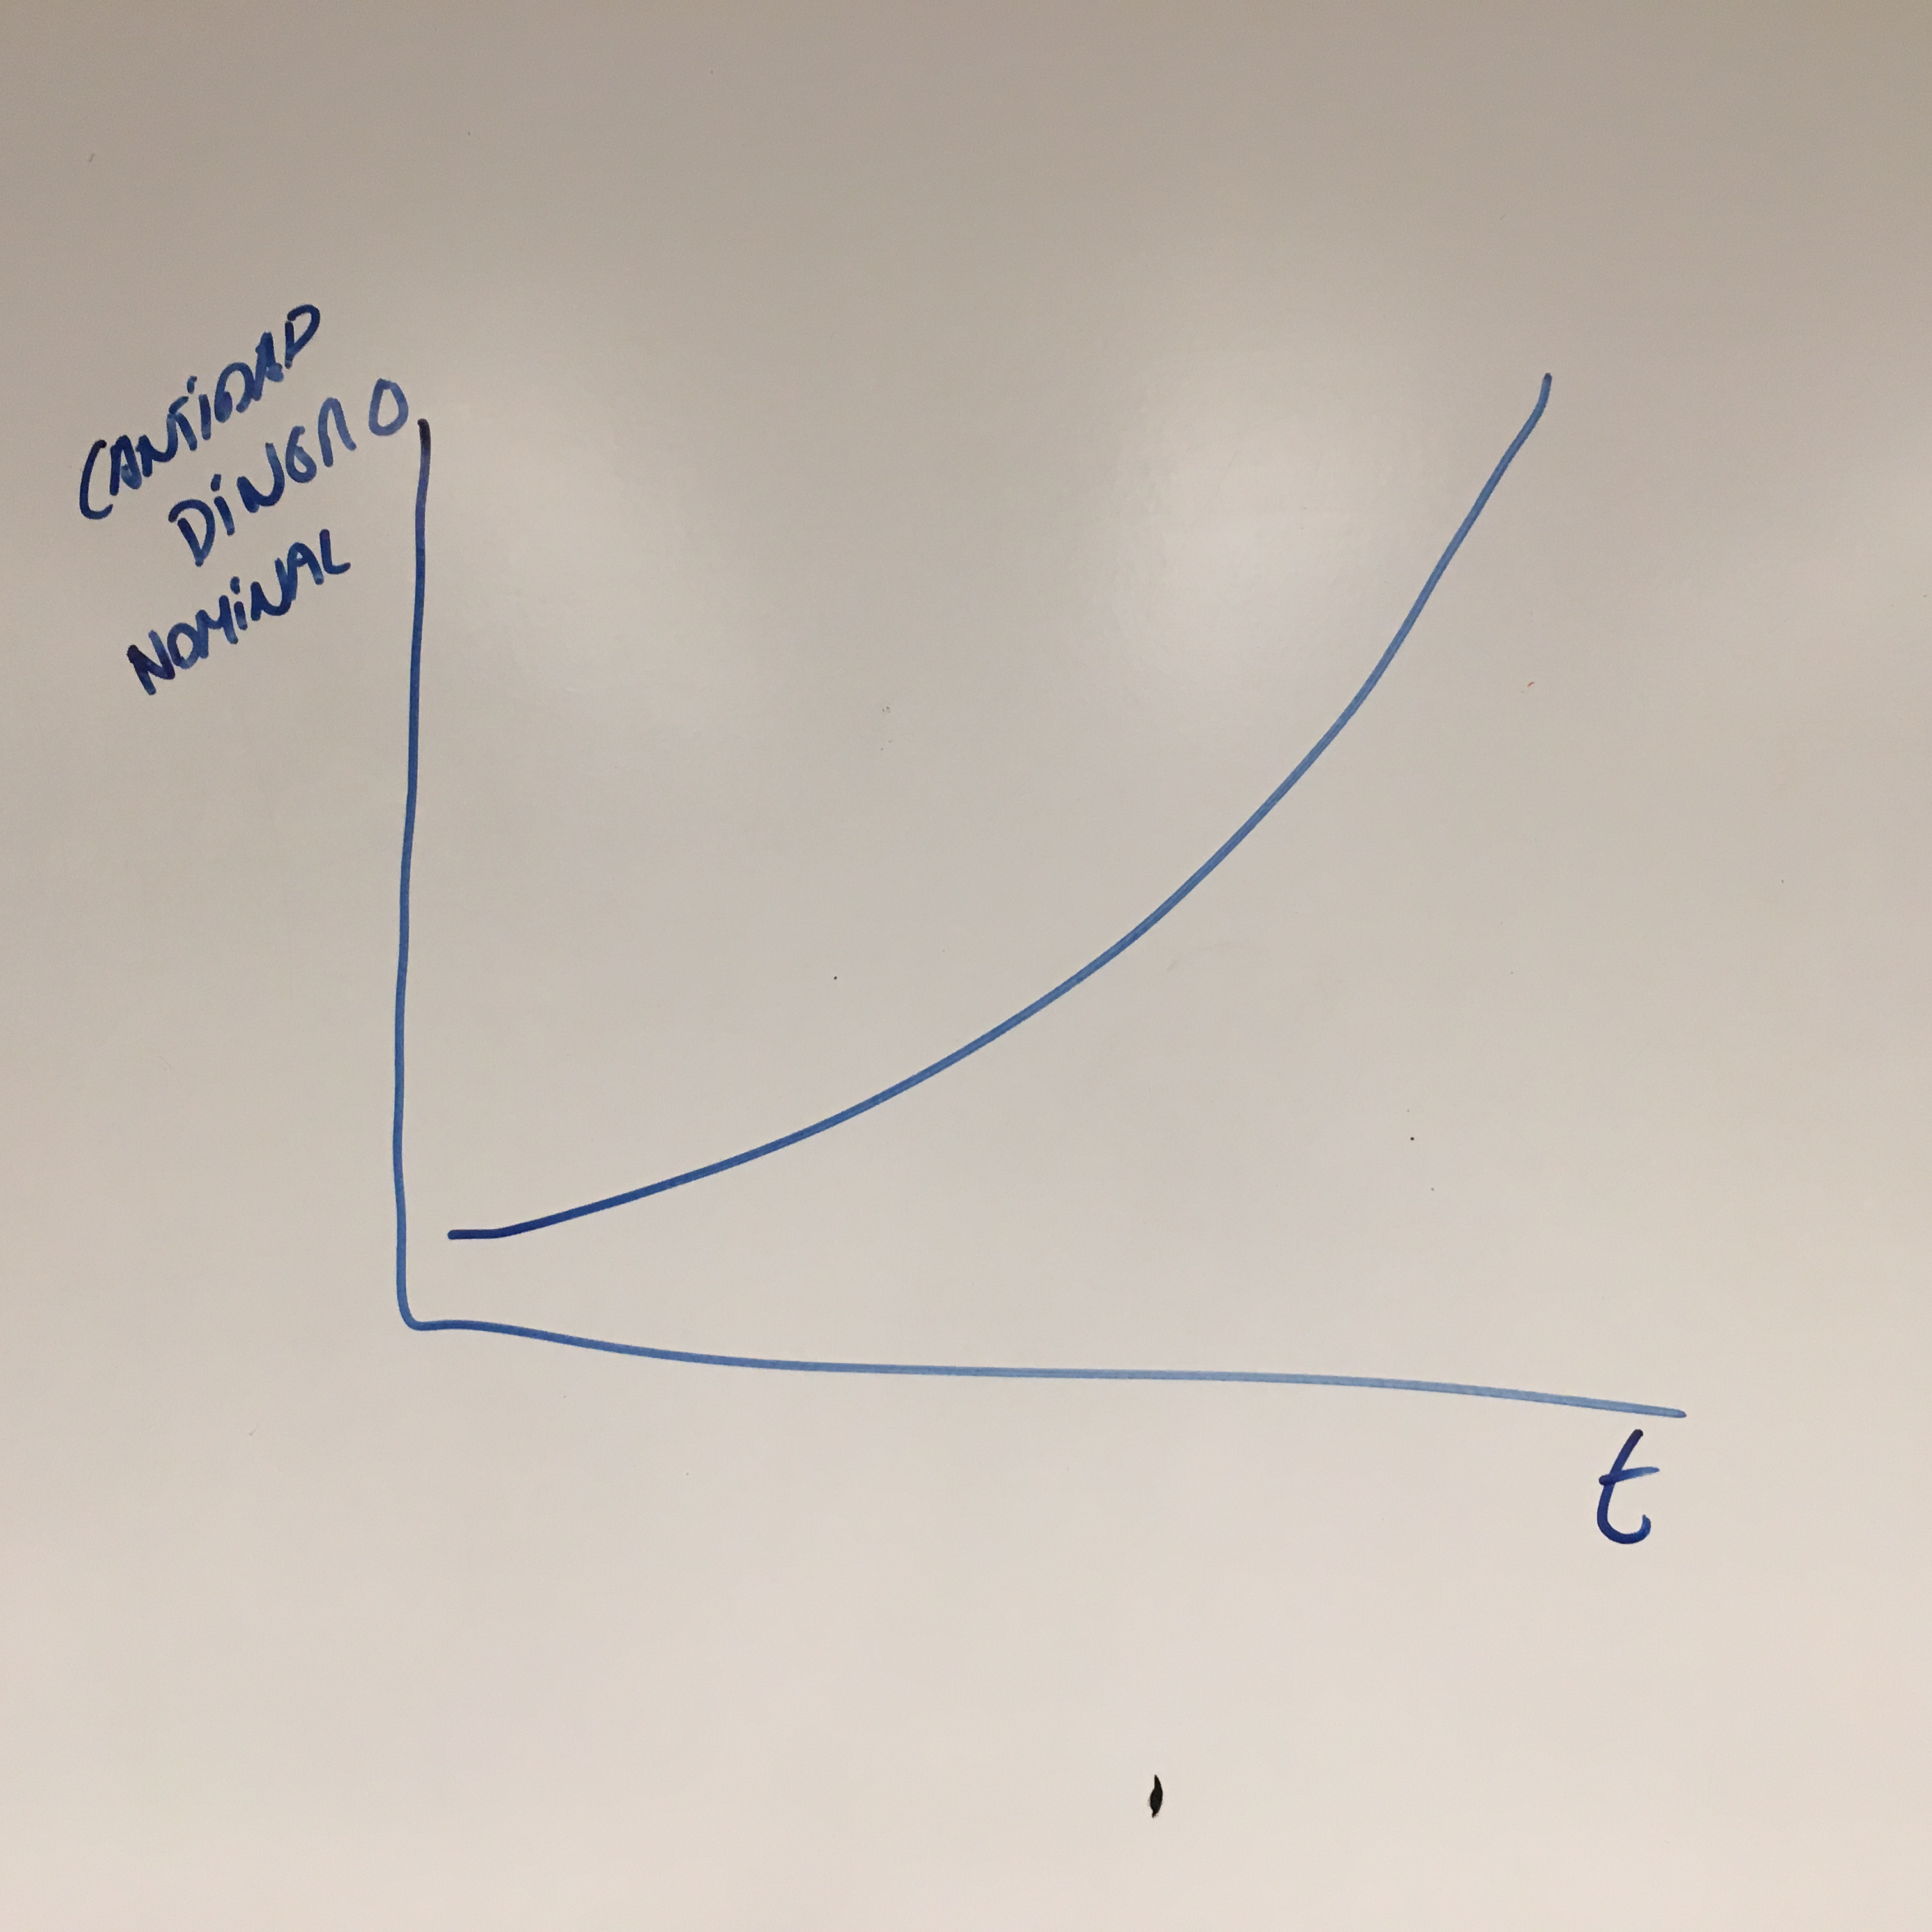
\includegraphics[width=6cm]{Classes/Images/2019-10-09_1.JPG}
                    \caption{El eje-x es tiempo, y el eje-y es la cantidad nominal de dinero}
                    \label{}
                \end{figure} 
                \begin{figure}[htbp]
                    \centering
                    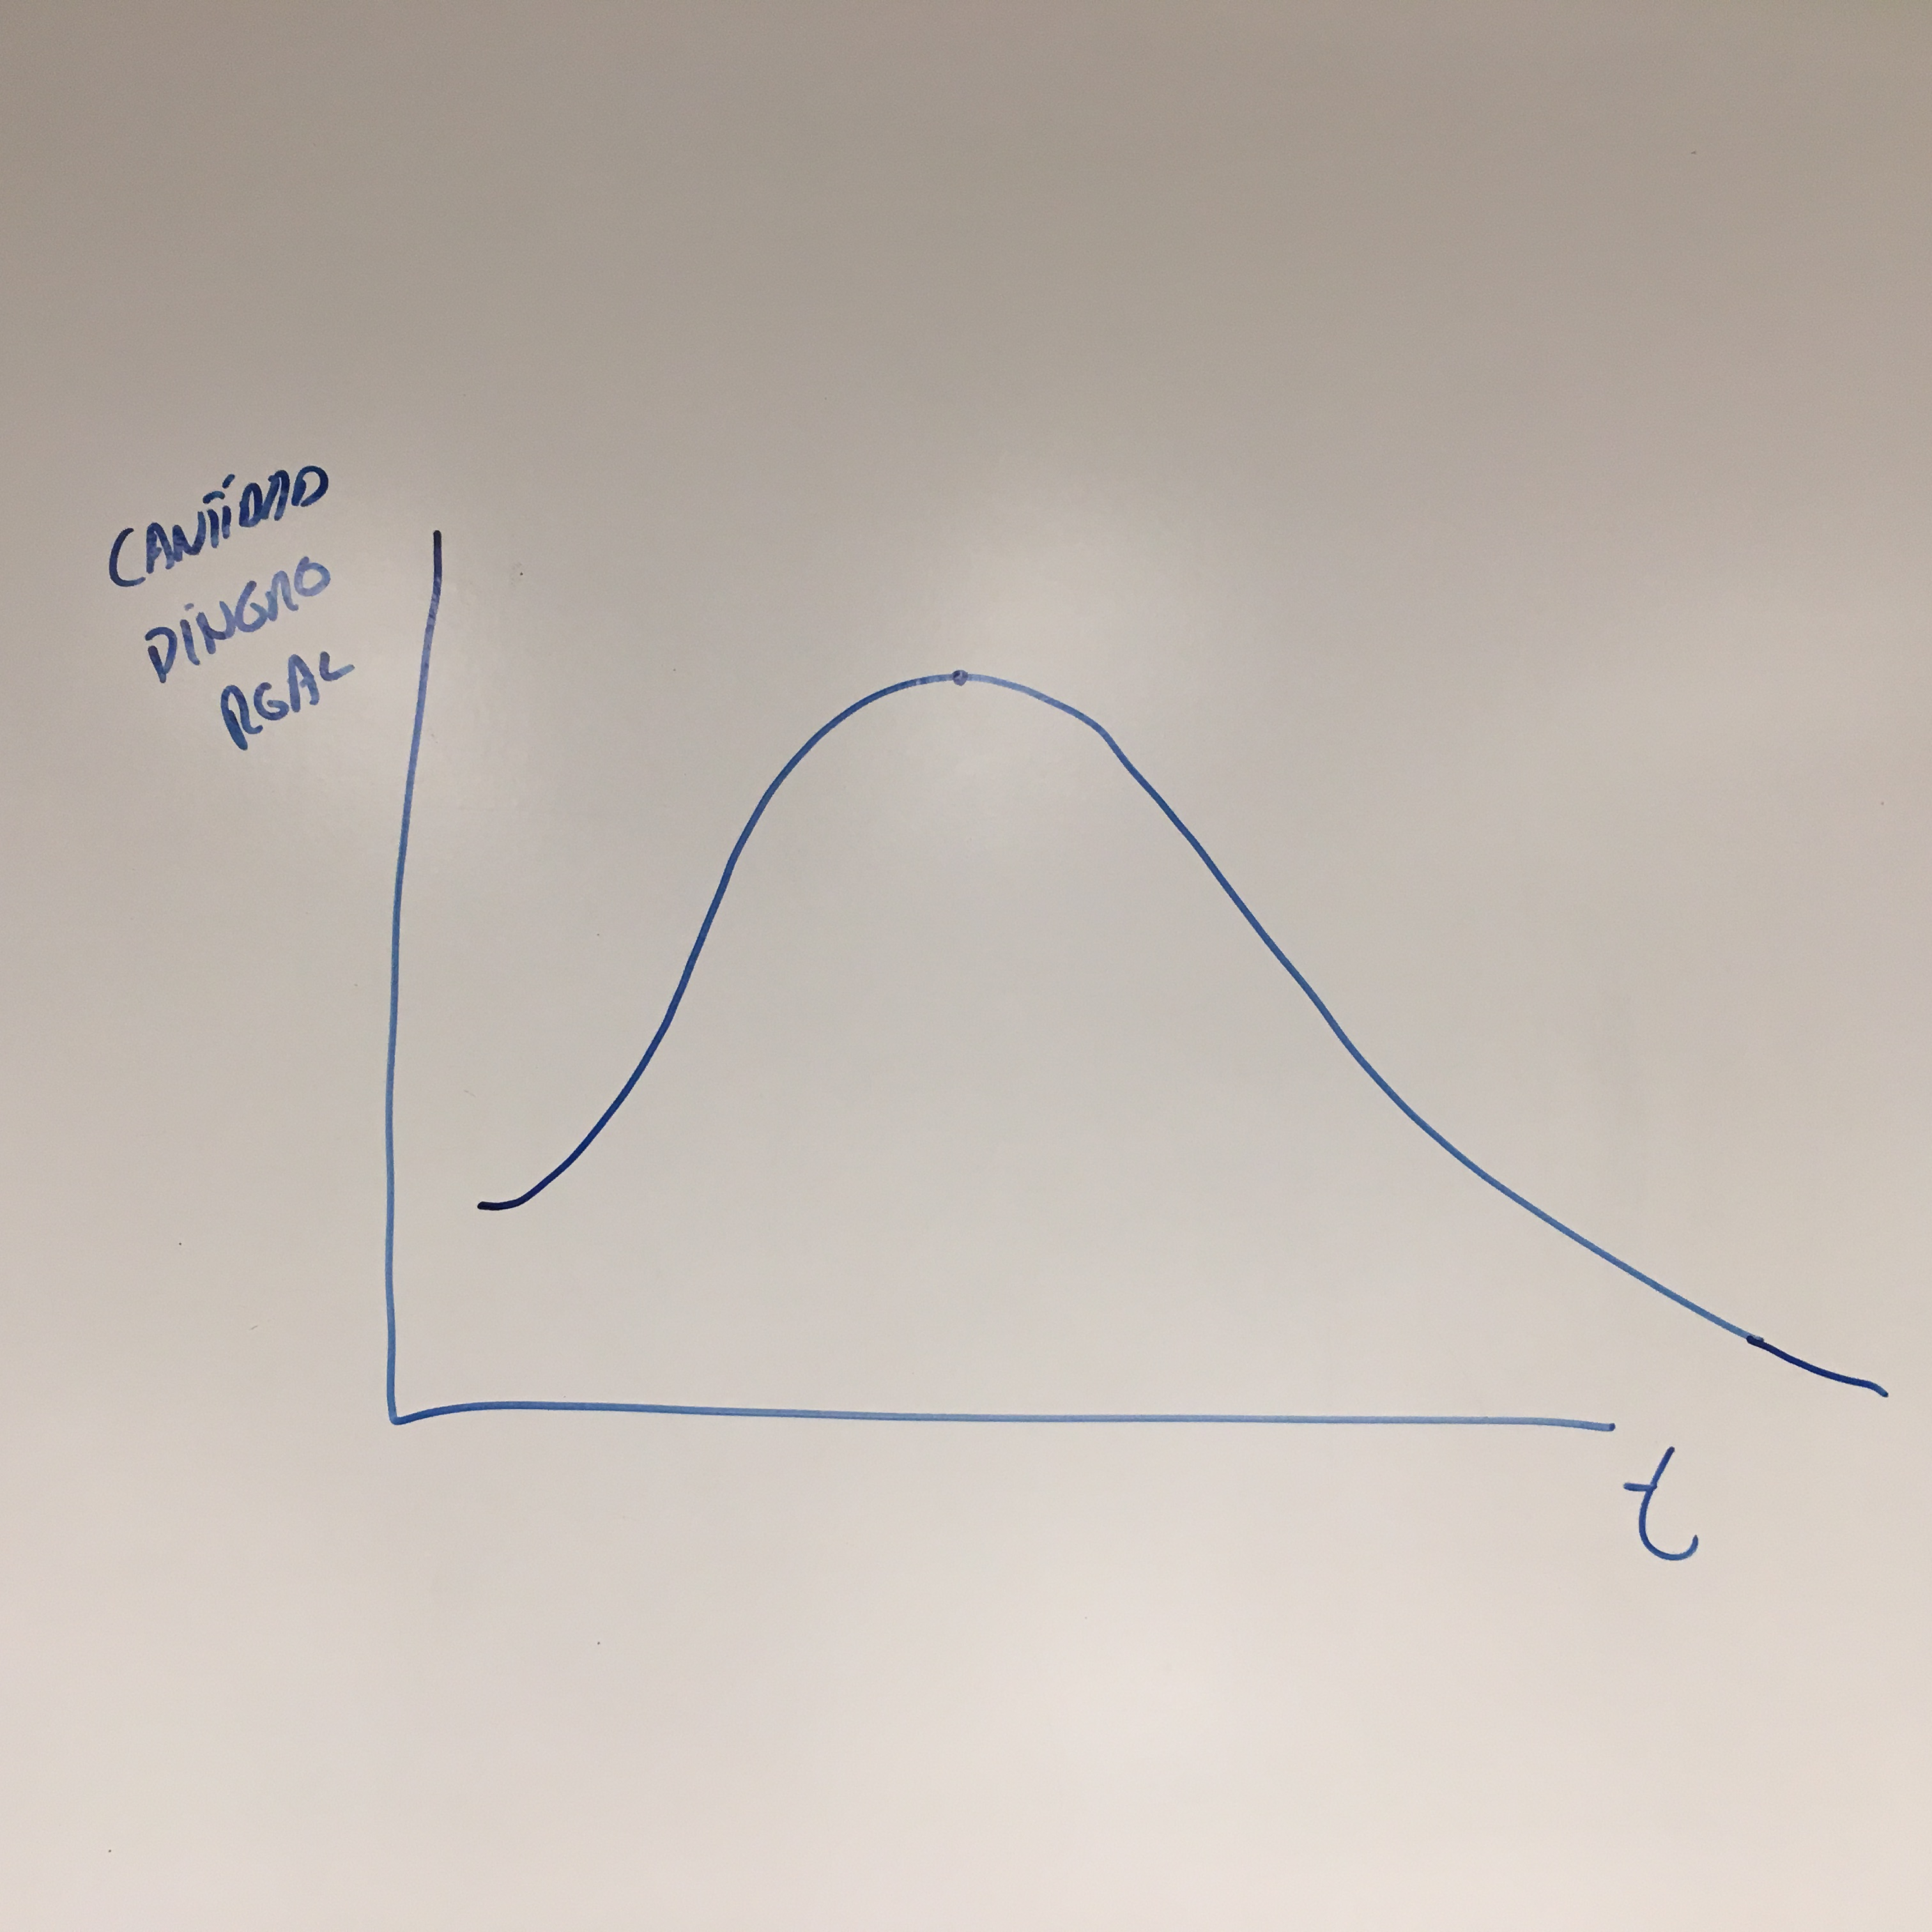
\includegraphics[width=6cm]{Classes/Images/2019-10-09_2.JPG}
                    \caption{El eje-x es tiempo, y el eje-y es la cantidad de dinero real}
                    \label{}
                \end{figure} 
            
            \item Considerar la siguiente fórmula para calcular:
                \[
                  \text{Oferta de dinero real} = \frac{\text{Oferta nominal}}{\text{Precios}}
                \]
            
            \item La demanda de dinero depende de la incertidumbre, cuando se siente que se va a depreciar la moneda todas las personas se quieren deshacer de la moneda por que los voy a perder, por eso se dice que la que tiende a circular la \textbf{buena moneda}. Considerar lo siguiente, en las hiper-inflaciones es de cobrar más amenudo \emph{\textbf{Ejemplo: }te cobran cada 15 minutos.}
            \item El punto de quiebre es cuando todos anticipan la depreciación de la moneda entonces se produce una escazes de dinero. 
        \end{itemize}
        
        \item Entonces el dinero es tan disfuncional que se vuelve a un trueque, se \textbf{rechaza} la moneda por completo. Se tiende a observar cosas como el barendero barriendo miles de millones en la divisa hiper-inflada por que es más valioso el papel que está hecho el dinero que el dinero en sí.
        \item \emph{\textbf{Ejemplo: }Venezuela y el precio del www.dollartoday.com es un sitio que se utiliza para averiguar el valor actual en Bolívares}.
        \item La ley de Thiers va a aplicar cuando la oferta de moneda sea mucho y pierde su función de medio de intercambio generalmente aceptado, en este momento se cumple la ley de Thiers por que ya no vale nada.
        \item \emph{Citación:``Siempre cuando exceda el punto de quiebe y la oferta del dinero real va en picada se aplica la ley de Thiers."}
        \item \emph{Citación:``Antes de la hiper-inflación iba con un poco de dinero y podía comprar una carreta de bienes, ahora voy con una carreta de dinero y regreso con un solo bien"}
        \item \emph{\textbf{Definición de ``punto de quiebre":} cuando el denominador  osea los precios son más grandes que la oferta real de dinero}
        \item Se puede hacer algo para revertir una hiperinflación si el gobierno se compromete se deprecian los precios, para hacer eso hay que  dejar de hacer déficit fiscal.
        \item \emph{\textbf{Ejemplo: }Venezuela no se dollariza por razones de nacionalismo}
        \item Dos indoles:
            \begin{enumerate}
                \item Índole 
                \item Índole bélica, cuando hay guerra siempre habrá un déficit fiscal, la salida o la forma de mobilizar grandes cantidades de recursos es aumentar la cantidad de dinero.
            \end{enumerate}
        
        \item \emph{\textbf{(Paréntesis ``paris como un foco de ideología'':}Siempre las ideas socialistas y de izquierda surgen de París  \textbf{)}} \emph{\textbf{Recordar lo siguiente:}Jermenes rojos, cuando juzgan este régimen ponen de escusas su adoctrinación en París de sus profesores marxistas.}
        \item \emph{Citación:``El camino al infierno está plagado de buenas intenciones"}
        \item En el manifiesto communista establece que para instituir un régimen socialista se debe de hacer hiper-inflación para quitarle todo el valor al dinero. 
        \item \emph{\textbf{Ejemplo: }hiper-inflación de beimar}
        \item Causas de una hiper-inflación: 
            \begin{enumerate}
                \item Ignorancia
                \item Socialismo o comunismo
            \end{enumerate}
        
        \item GT es un país estable por que el gobierno no tiene control en el banco central.
\end{enumerate}
